\documentclass[12pt]{report}
\usepackage{amsmath,amsthm,latexsym,paralist}
\usepackage[document]{ragged2e}
\usepackage{tikz}

\theoremstyle{definition}
\newtheorem{problem}{Problem}

\begin{document}

\vspace*{-15mm}
\begin{center}
{\large
				CSCE 221 - Homework Set 9 \\
				Due 5/5/2015, 11:59 PM}
\end{center}

\begin{problem} R-13.1 (15 points)
\end{problem}

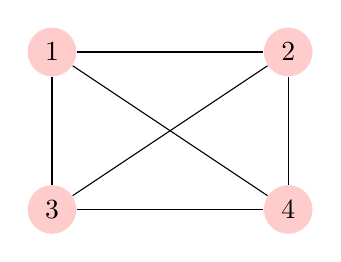
\begin{tikzpicture}[scale=1,auto=left,every node/.style={circle,fill=red!20}]
	\node (n1) at (1,10) {1};
	\node (n2) at (4,10) {2};
	\node (n3) at (1,8) {3};
	\node (n4) at (4,8) {4};
	\foreach \from/\to in {n1/n2,n1/n3,n2/n3,n1/n4,n2/n4,n3/n4}
		\draw (\from) -- (\to);
\end{tikzpicture}

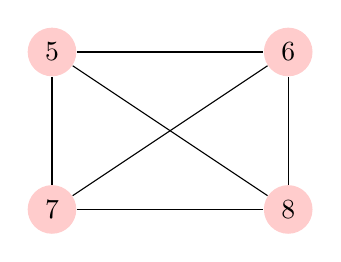
\begin{tikzpicture}[scale=1,auto=left,every node/.style={circle,fill=red!20}]
	\node (n1) at (1,10) {5};
	\node (n2) at (4,10) {6};
	\node (n3) at (1,8) {7};
	\node (n4) at (4,8) {8};
	\foreach \from/\to in {n1/n2,n1/n3,n2/n3,n1/n4,n2/n4,n3/n4}
		\draw (\from) -- (\to);
\end{tikzpicture}

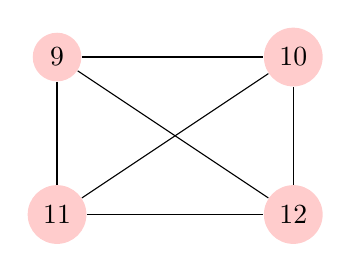
\begin{tikzpicture}[scale=1,auto=left,every node/.style={circle,fill=red!20}]
	\node (n1) at (1,10) {9};
	\node (n2) at (4,10) {10};
	\node (n3) at (1,8) {11};
	\node (n4) at (4,8) {12};
	\foreach \from/\to in {n1/n2,n1/n3,n2/n3,n1/n4,n2/n4,n3/n4}
		\draw (\from) -- (\to);
\end{tikzpicture}

It is possible to draw a graph with 12 verticies and 66 edges, but it's impossible to draw a graph with 66 edges and 3 connected components. For any undirected graph with $n$ verticies and $m$ edges,  $m \le \dfrac{n(n-1)}{2}$. Thus, a graph having 3 connected components would yield a max of 30 edges, according to this theorem, proving it impossible if the graph had 66 edges.

\begin{problem} R-13.2 (20 points)
\end{problem}

\begin{problem} R-13.7 (21 points)
\end{problem}

\begin{problem} R-13.8 (15 points)
\end{problem}

\begin{problem} R-13.9 (10 points)
\end{problem}

\begin{problem} R-13.13 (20 points)
\end{problem}

\begin{problem} R-13.21 (15 points)
\end{problem}

\begin{problem} R-13.22 (15 points)
\end{problem}

\end{document}